% Copyright 2017 Emilio Rojas
%
% Permission is hereby granted, free of charge, to any person obtaining a copy of
% this software and associated documentation files (the "Software"), to deal in
% the Software without restriction, including without limitation the rights to
% use, copy, modify, merge, publish, distribute, sublicense, and/or sell copies of
% the Software, and to permit persons to whom the Software is furnished to do so,
% subject to the following conditions:
%
% The above copyright notice and this permission notice shall be included in all
% copies or substantial portions of the Software.
%
% THE SOFTWARE IS PROVIDED "AS IS", WITHOUT WARRANTY OF ANY KIND, EXPRESS OR
% IMPLIED, INCLUDING BUT NOT LIMITED TO THE WARRANTIES OF MERCHANTABILITY, FITNESS
% FOR A PARTICULAR PURPOSE AND NONINFRINGEMENT. IN NO EVENT SHALL THE AUTHORS OR
% COPYRIGHT HOLDERS BE LIABLE FOR ANY CLAIM, DAMAGES OR OTHER LIABILITY, WHETHER
% IN AN ACTION OF CONTRACT, TORT OR OTHERWISE, ARISING FROM, OUT OF OR IN
% CONNECTION WITH THE SOFTWARE OR THE USE OR OTHER DEALINGS IN THE SOFTWARE.

\documentclass{article}

% Copyright 2017 Emilio Rojas
%
% Permission is hereby granted, free of charge, to any person obtaining a copy of
% this software and associated documentation files (the "Software"), to deal in
% the Software without restriction, including without limitation the rights to
% use, copy, modify, merge, publish, distribute, sublicense, and/or sell copies of
% the Software, and to permit persons to whom the Software is furnished to do so,
% subject to the following conditions:
%
% The above copyright notice and this permission notice shall be included in all
% copies or substantial portions of the Software.
%
% THE SOFTWARE IS PROVIDED "AS IS", WITHOUT WARRANTY OF ANY KIND, EXPRESS OR
% IMPLIED, INCLUDING BUT NOT LIMITED TO THE WARRANTIES OF MERCHANTABILITY, FITNESS
% FOR A PARTICULAR PURPOSE AND NONINFRINGEMENT. IN NO EVENT SHALL THE AUTHORS OR
% COPYRIGHT HOLDERS BE LIABLE FOR ANY CLAIM, DAMAGES OR OTHER LIABILITY, WHETHER
% IN AN ACTION OF CONTRACT, TORT OR OTHERWISE, ARISING FROM, OUT OF OR IN
% CONNECTION WITH THE SOFTWARE OR THE USE OR OTHER DEALINGS IN THE SOFTWARE.

% Estos son los paquetes que se cargan en todos los documentos, estos paquetes
% están en texlive-full (TODO separar paquetes por seccion de texlive donde
% está el paqeute). De momento se ordenan por longitud del nombre y
% alfabeticamente.

\usepackage{url}
\usepackage{cite}
\usepackage{tikz}

\usepackage{array}
\usepackage{color}
\usepackage{float}

\usepackage{empheq}

\usepackage{amsmath}
\usepackage{apacite}
\usepackage{caption}
\usepackage{gensymb}
\usepackage{siunitx}

\usepackage{amsfonts}
\usepackage{booktabs}
\usepackage{enumitem}
\usepackage{etoolbox}
\usepackage{fancyhdr}
\usepackage{graphicx}
\usepackage{geometry}
\usepackage{hyperref}
\usepackage{mdframed}
\usepackage{multirow}
\usepackage{pdfpages}
\usepackage{pgfplots}
\usepackage{setspace}
\usepackage{textcomp}

\usepackage{adjustbox}
\usepackage{mathtools}

\usepackage{circuitikz}
\usepackage{subcaption}

\usepackage[T1]{fontenc}
\usepackage[spanish]{babel}
\usepackage[utf8]{inputenc}


%%http://tex.stackexchange.com/questions/140567/drawing-karnaughs-maps-in-latex
\usetikzlibrary{matrix, calc}

%isolated term
%#1 - Optional. Space between node and grouping line. Default=0
%#2 - node
%#3 - filling color
\newcommand{\implicantsol}[3][0]{
  \draw[rounded corners=3pt, fill=#3, opacity=0.3] ($(#2.north west)+(135:#1)$) rectangle ($(#2.south east)+(-45:#1)$);
}


%internal group
%#1 - Optional. Space between node and grouping line. Default=0
%#2 - top left node
%#3 - bottom right node
%#4 - filling color
\newcommand{\implicant}[4][0]{
  \draw[rounded corners=3pt, fill=#4, opacity=0.3] ($(#2.north west)+(135:#1)$) rectangle ($(#3.south east)+(-45:#1)$);
}

%group lateral borders
%#1 - Optional. Space between node and grouping line. Default=0
%#2 - top left node
%#3 - bottom right node
%#4 - filling color
\newcommand{\implicantcostats}[4][0]{
  \draw[rounded corners=3pt, fill=#4, opacity=0.3] ($(rf.east |- #2.north)+(90:#1)$)-| ($(#2.east)+(0:#1)$) |- ($(rf.east |- #3.south)+(-90:#1)$);
  \draw[rounded corners=3pt, fill=#4, opacity=0.3] ($(cf.west |- #2.north)+(90:#1)$) -| ($(#3.west)+(180:#1)$) |- ($(cf.west |- #3.south)+(-90:#1)$);
}

%group top-bottom borders
%#1 - Optional. Space between node and grouping line. Default=0
%#2 - top left node
%#3 - bottom right node
%#4 - filling color
\newcommand{\implicantdaltbaix}[4][0]{
  \draw[rounded corners=3pt, fill=#4, opacity=0.3] ($(cf.south -| #2.west)+(180:#1)$) |- ($(#2.south)+(-90:#1)$) -| ($(cf.south -| #3.east)+(0:#1)$);
  \draw[rounded corners=3pt, fill=#4, opacity=0.3] ($(rf.north -| #2.west)+(180:#1)$) |- ($(#3.north)+(90:#1)$) -| ($(rf.north -| #3.east)+(0:#1)$);
}

%group corners
%#1 - Optional. Space between node and grouping line. Default=0
%#2 - filling color
\newcommand{\implicantcantons}[2][0]{
  \draw[rounded corners=3pt, opacity=.3] ($(rf.east |- 0.south)+(-90:#1)$) -| ($(0.east |- cf.south)+(0:#1)$);
  \draw[rounded corners=3pt, opacity=.3] ($(rf.east |- 8.north)+(90:#1)$) -| ($(8.east |- rf.north)+(0:#1)$);
  \draw[rounded corners=3pt, opacity=.3] ($(cf.west |- 2.south)+(-90:#1)$) -| ($(2.west |- cf.south)+(180:#1)$);
  \draw[rounded corners=3pt, opacity=.3] ($(cf.west |- 10.north)+(90:#1)$) -| ($(10.west |- rf.north)+(180:#1)$);
  \fill[rounded corners=3pt, fill=#2, opacity=.3] ($(rf.east |- 0.south)+(-90:#1)$) -|  ($(0.east |- cf.south)+(0:#1)$) [sharp corners] ($(rf.east |- 0.south)+(-90:#1)$) |-  ($(0.east |- cf.south)+(0:#1)$) ;
  \fill[rounded corners=3pt, fill=#2, opacity=.3] ($(rf.east |- 8.north)+(90:#1)$) -| ($(8.east |- rf.north)+(0:#1)$) [sharp corners] ($(rf.east |- 8.north)+(90:#1)$) |- ($(8.east |- rf.north)+(0:#1)$) ;
  \fill[rounded corners=3pt, fill=#2, opacity=.3] ($(cf.west |- 2.south)+(-90:#1)$) -| ($(2.west |- cf.south)+(180:#1)$) [sharp corners]($(cf.west |- 2.south)+(-90:#1)$) |- ($(2.west |- cf.south)+(180:#1)$) ;
  \fill[rounded corners=3pt, fill=#2, opacity=.3] ($(cf.west |- 10.north)+(90:#1)$) -| ($(10.west |- rf.north)+(180:#1)$) [sharp corners] ($(cf.west |- 10.north)+(90:#1)$) |- ($(10.west |- rf.north)+(180:#1)$) ;
}

%Empty Karnaugh map 4x4
\newenvironment{Karnaugh}[4]%
{
  \begin{tikzpicture}[baseline=(current bounding box.north),scale=0.8]
    \draw (0,0) grid (4,4);
    \draw[very thick] (-0.3, 0) -- node[left] {#1} ++(0, 2);
    \draw[very thick] (4.3, 1) -- node[right] {#2} ++(0, 2);
    \draw[very thick] (2, 4.3) -- node [above] {#3} ++(2, 0);
    \draw[very thick] (1, -0.3) -- node [below] {#4 } ++(2, 0);
    %
    \matrix (mapa) [matrix of nodes,
      column sep={0.8cm,between origins},
      row sep={0.8cm,between origins},
      every node/.style={minimum size=0.3mm},
      anchor=8.center,
    ampersand replacement=\&] at (0.5,0.5)
    {
      \& |(c00)|            \& |(c01)|            \& |(c11)|            \& |(c10)|            \& |(cf)| \phantom{00} \\
      |(r00)|                \& |(0)|  \phantom{0} \& |(1)|  \phantom{0} \& |(3)|  \phantom{0} \& |(2)|  \phantom{0} \&                     \\
      |(r01)|                \& |(4)|  \phantom{0} \& |(5)|  \phantom{0} \& |(7)|  \phantom{0} \& |(6)|  \phantom{0} \&                     \\
      |(r11)|                \& |(12)| \phantom{0} \& |(13)| \phantom{0} \& |(15)| \phantom{0} \& |(14)| \phantom{0} \&                     \\
      |(r10)|                \& |(8)|  \phantom{0} \& |(9)|  \phantom{0} \& |(11)| \phantom{0} \& |(10)| \phantom{0} \&                     \\
      |(rf) | \phantom{00}   \&                    \&                    \&                    \&                    \&                     \\
    };
  }%
  {
  \end{tikzpicture}
}

%Empty Karnaugh map 2x4
\newenvironment{Karnaughvuit}%
{
  \begin{tikzpicture}[baseline=(current bounding box.north),scale=0.8]
    \draw (0,0) grid (4,2);
    \draw (0,2) -- node [pos=0.7,above right,anchor=south west] {bc} node [pos=0.7,below left,anchor=north east] {a} ++(135:1);
    %
    \matrix (mapa) [matrix of nodes,
      column sep={0.8cm,between origins},
      row sep={0.8cm,between origins},
      every node/.style={minimum size=0.3mm},
      anchor=4.center,
    ampersand replacement=\&] at (0.5,0.5)
    {
      \& |(c00)| 00         \& |(c01)| 01         \& |(c11)| 11         \& |(c10)| 10         \& |(cf)| \phantom{00} \\
      |(r00)| 0             \& |(0)|  \phantom{0} \& |(1)|  \phantom{0} \& |(3)|  \phantom{0} \& |(2)|  \phantom{0} \&                     \\
      |(r01)| 1             \& |(4)|  \phantom{0} \& |(5)|  \phantom{0} \& |(7)|  \phantom{0} \& |(6)|  \phantom{0} \&                     \\
      |(rf) | \phantom{00}  \&                    \&                    \&                    \&                    \&                     \\
    };
  }%
  {
  \end{tikzpicture}
}

%Empty Karnaugh map 2x2
\newenvironment{Karnaughquatre}%
{
  \begin{tikzpicture}[baseline=(current bounding box.north),scale=0.8]
    \draw (0,0) grid (2,2);
    \draw (0,2) -- node [pos=0.7,above right,anchor=south west] {b} node [pos=0.7,below left,anchor=north east] {a} ++(135:1);
    %
    \matrix (mapa) [matrix of nodes,
      column sep={0.8cm,between origins},
      row sep={0.8cm,between origins},
      every node/.style={minimum size=0.3mm},
      anchor=2.center,
    ampersand replacement=\&] at (0.5,0.5)
    {
      \& |(c00)| 0          \& |(c01)| 1  \\
      |(r00)| 0 \& |(0)|  \phantom{0} \& |(1)|  \phantom{0} \\
      |(r01)| 1 \& |(2)|  \phantom{0} \& |(3)|  \phantom{0} \\
    };
  }%
  {
  \end{tikzpicture}
}

%Defines 8 or 16 values (0,1,X)
\newcommand{\contingut}[1]{%
  \foreach \x [count=\xi from 0]  in {#1}
  \path (\xi) node {\x};
}

%Places 1 in listed positions
\newcommand{\minterms}[1]{%
  \foreach \x in {#1}
  \path (\x) node {1};
}

%Places 0 in listed positions
\newcommand{\maxterms}[1]{%
  \foreach \x in {#1}
  \path (\x) node {0};
}

%Places X in listed positions
\newcommand{\indeterminats}[1]{%
  \foreach \x in {#1}
  \path (\x) node {X};
}

% Copyright 2017 Emilio Rojas
%
% Permission is hereby granted, free of charge, to any person obtaining a copy of
% this software and associated documentation files (the "Software"), to deal in
% the Software without restriction, including without limitation the rights to
% use, copy, modify, merge, publish, distribute, sublicense, and/or sell copies of
% the Software, and to permit persons to whom the Software is furnished to do so,
% subject to the following conditions:
%
% The above copyright notice and this permission notice shall be included in all
% copies or substantial portions of the Software.
%
% THE SOFTWARE IS PROVIDED "AS IS", WITHOUT WARRANTY OF ANY KIND, EXPRESS OR
% IMPLIED, INCLUDING BUT NOT LIMITED TO THE WARRANTIES OF MERCHANTABILITY, FITNESS
% FOR A PARTICULAR PURPOSE AND NONINFRINGEMENT. IN NO EVENT SHALL THE AUTHORS OR
% COPYRIGHT HOLDERS BE LIABLE FOR ANY CLAIM, DAMAGES OR OTHER LIABILITY, WHETHER
% IN AN ACTION OF CONTRACT, TORT OR OTHERWISE, ARISING FROM, OUT OF OR IN
% CONNECTION WITH THE SOFTWARE OR THE USE OR OTHER DEALINGS IN THE SOFTWARE.

% allows to use < and > on tikz pictures when babel set to spanish
% http://tex.stackexchange.com/questions/166772/problem-with-babel-and-tikz-using-draw
\usetikzlibrary{babel}
\usetikzlibrary{positioning}
\usetikzlibrary{quotes, angles}

\pgfplotsset{compat=1.13}

\setlength
  {\columnsep}
  {1cm}

\patchcmd
  {\chapter}
  {\thispagestyle{plain}}
  {\thispagestyle{fancy}}
  {}
  {}

\geometry
  {
    a4paper,
    left=25.4mm,
    right=25.4mm,
    top=25.4mm,
    bottom=25.4mm,
    heightrounded,
  }

\sisetup{output-exponent-marker=\textsc{e}}
\setlength{\jot}{10pt}

% FANCY SETTINGS
\pagestyle{fancy}
\fancyhf{}
\lhead{Circuitos Digitales I}
\rfoot{\thepage}
\setlength{\headheight}{20pt}

% ZENER
\makeatletter
\pgfcircdeclarebipole{}{
  \ctikzvalof{bipoles/diode/height}
}{fullzzdiode}{
  \ctikzvalof{bipoles/diode/height}
}{
  \ctikzvalof{bipoles/diode/width}
}{

  \pgfsetlinewidth{\pgfkeysvalueof{/tikz/circuitikz/bipoles/thickness}\pgfstartlinewidth}

  \pgfscope
    \pgftransformxshift{\pgf@circ@res@left}
    \pgfpathmoveto{\pgfpoint{\pgf@circ@res@right-\pgf@circ@res@left}{0pt}}
    \pgfpathlineto{\pgfpoint{0pt}{\pgf@circ@res@up}}
    \pgfpathlineto{\pgfpoint{0pt}{\pgf@circ@res@down}}
    \pgfpathlineto{\pgfpoint{\pgf@circ@res@right-\pgf@circ@res@left}{0pt}}
    \pgfusepath{draw,fill}
    \pgfpathmoveto{
      \pgfpoint{
        \pgf@circ@res@right-1.8\pgf@circ@res@left
      }{
        \pgf@circ@res@down-0.5\pgf@circ@res@up
      }
    }
    \pgfpathlineto{
      \pgfpoint{
        \pgf@circ@res@right-\pgf@circ@res@left
      }{
        \pgf@circ@res@down
      }
    }
    \pgfpathlineto{
      \pgfpoint{
        \pgf@circ@res@right-\pgf@circ@res@left
      }{
        \pgf@circ@res@up
      }
    }
    \pgfpathlineto{
      \pgfpoint{
        \pgf@circ@res@right-0.2\pgf@circ@res@left
      }{
        \pgf@circ@res@up-0.5\pgf@circ@res@down
      }
    }
    \pgfusepath{draw}
  \endpgfscope
}
\def\pgf@circ@fullzzdiode@path#1{\pgf@circ@bipole@path{fullzzdiode}{#1}}
\tikzset{full Zzener diode/.style = {\circuitikzbasekey, /tikz/to path=\pgf@circ@fullzzdiode@path}}
\tikzset{zzD*/.style = {full Zzener diode}}
\makeatother

% Copyright 2017 Emilio Rojas
%
% Permission is hereby granted, free of charge, to any person obtaining a copy of
% this software and associated documentation files (the "Software"), to deal in
% the Software without restriction, including without limitation the rights to
% use, copy, modify, merge, publish, distribute, sublicense, and/or sell copies of
% the Software, and to permit persons to whom the Software is furnished to do so,
% subject to the following conditions:
%
% The above copyright notice and this permission notice shall be included in all
% copies or substantial portions of the Software.
%
% THE SOFTWARE IS PROVIDED "AS IS", WITHOUT WARRANTY OF ANY KIND, EXPRESS OR
% IMPLIED, INCLUDING BUT NOT LIMITED TO THE WARRANTIES OF MERCHANTABILITY, FITNESS
% FOR A PARTICULAR PURPOSE AND NONINFRINGEMENT. IN NO EVENT SHALL THE AUTHORS OR
% COPYRIGHT HOLDERS BE LIABLE FOR ANY CLAIM, DAMAGES OR OTHER LIABILITY, WHETHER
% IN AN ACTION OF CONTRACT, TORT OR OTHERWISE, ARISING FROM, OUT OF OR IN
% CONNECTION WITH THE SOFTWARE OR THE USE OR OTHER DEALINGS IN THE SOFTWARE.

% Unnumbered section added to toc
% 1: The section's name.
\newcommand{\usection}[1]
{
  \section*{#1}
  \addcontentsline{toc}{section}{#1}
}

% Unnumbered subsection added to toc
% 1: The subsection's name.
\newcommand{\usubsection}[1]
{
  \subsection*{#1}
  \addcontentsline{toc}{subsection}{#1}
}

% Unnumbered subsubsection added to toc
% 1: The subsubsection's name.
\newcommand{\usubsubsection}[1]
{
  \subsubsection*{#1}
  \addcontentsline{toc}{subsubsection}{#1}
}

% Uncut table rules
\makeatletter
\newlength\mylena
\newlength\mylenb
\newcommand\mystrut[1][2]{%
    \setlength\mylena{#1\ht\@arstrutbox}%
    \setlength\mylenb{#1\dp\@arstrutbox}%
    \rule[\mylenb]{0pt}{\mylena}}
\makeatother

% Circuitikz equal
\newcommand*{\equal}{=}

% Adds a title page to the document
% 1: The document's name
% 2: The document's owner's name
% 3: The document's owner's id
% 4: The document's date

% \portada{Homework}{John Doe}{123456}{\today}
\newcommand{\portada}[4]
{
  \begin{titlepage}
    \vspace*{\fill}
    \begin{center}

      \textsc{\Large Universidad de Costa Rica}\\
      [0.25in]

      \textsc{\Large Escuela de Ingeniería Eléctrica}\\
      [0.55in]

      \textsc{\Large Circuitos Digitales I - IE0323}\\
      [0.25in]

      \textsc{\huge \bfseries {#1}}\\
      [0.5in]

      \textsc{\large {#2}}\\
      \textsc{\large {#3}}\\
      [0.5in]

      \textsc{\large {#4}}
    \end{center}
    \vspace*{\fill}
  \end{titlepage}
}


\begin{document}

\pagenumbering{gobble}

\portada
{Tarea \#4}
{Emilio Javier Rojas Álvarez}
{B15680}
{\today}


Se construye el siguiente circuito:
\begin{figure}[H]
  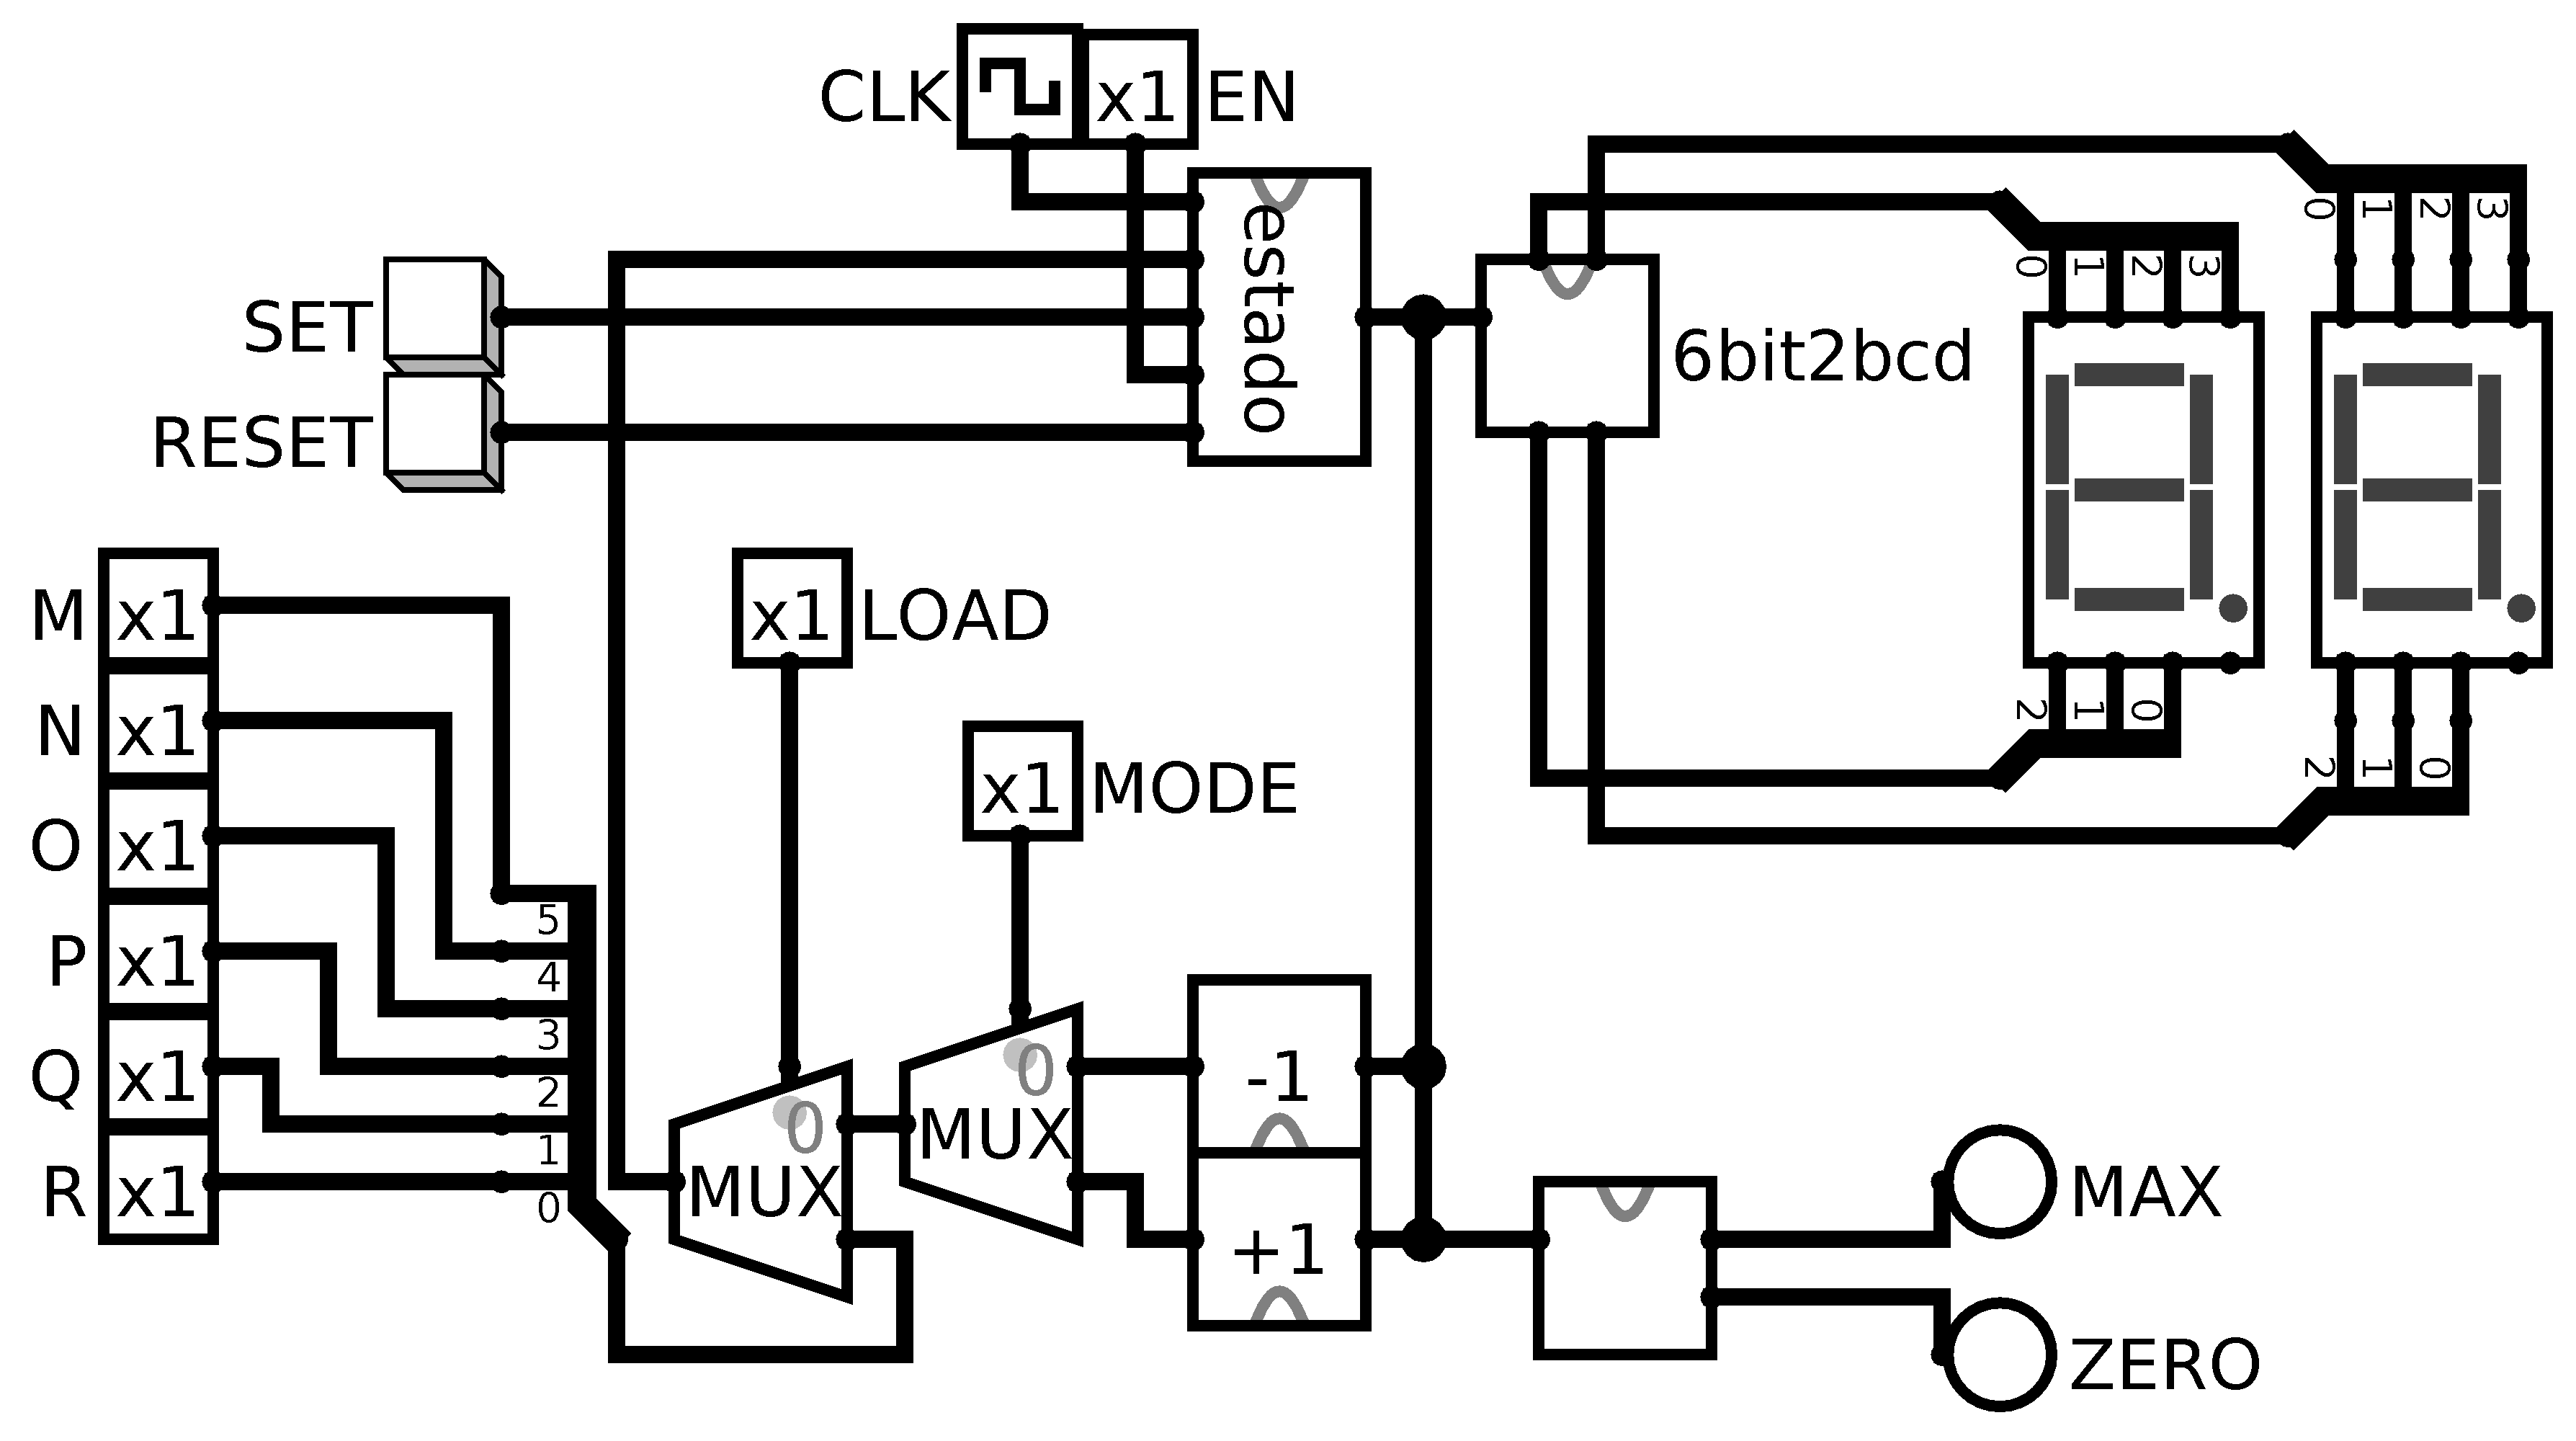
\includegraphics[width=\textwidth]{circuito/main.png}
  \caption{Bloques del contador.}
\end{figure}
El bloque \textit{estado} es un banco de 6 flip flops, cada uno contiene el
estado presente de uno de los bits en el contador. A este le entra una señal de
reloj, una de set(pone todos los bits en 1), una de reset(pone todos los bits en
0), una para indicar si se puede o no alterar el valor que almacena el flip
flop, y la entrada de datos. El bloque \textit{6bit2bcd} convierte la señal de 6
bits a 14 salidas para 2 pantallas de 7 segmentos que representan el número de
la señal.

Se identifican mediante 2 bombillos si el contador está en 0 o el número máximo.
Se tienen dos bloques, \textit{-1} y \textit{+1} que suman o restan 1 al estado
presente del contador. Estas cajas se obtienen a partir de mapas de Karnaugh.

Mediante MUXES se selecciona la señal de 6 bits que indicará el próximo flanco
de reloj. Esta puede ser una de 3, una señal MNOPQR que se activa con LOAD, el
siguiente número, cuando MODE está activo y LOAD inactivo o bien el número
previo cuando MODE y LOAD estén inactivos.



\usection{Contador Ascendente}
\begin{table}[H]
  \centering
  \begin{adjustbox}{max width=\textwidth}
    \begin{tabular}{ c | c | c | c | c | c | c ||| c | c | c | c | c | c || c | c | c | c | c | c }
       & \multicolumn{6}{c}{\textbf{Número Presente}} &
       \multicolumn{6}{c}{\textbf{Número Previo} \small{$Q_5=0$}} &
       \multicolumn{6}{c}{\textbf{Número Previo} \small{$Q_5=1$}} \\
      \toprule
      Decimal  &
      $Q_5$ & $Q_4$ & $Q_3$ & $Q_2$ & $Q_1$ & $Q_0$ &
      $Q_5\prime$ & $Q_4\prime$ & $Q_3\prime$ & $Q_2\prime$ & $Q_1\prime$ & $Q_0\prime$ &
      $Q_5\prime$ & $Q_4\prime$ & $Q_3\prime$ & $Q_2\prime$ & $Q_1\prime$ & $Q_0\prime$ \\
      \toprule
      %       Q5    Q4  Q3  Q2  Q1  Q0    Q5  Q4  Q3  Q2  Q1  Q0    Q5  Q4  Q3  Q2  Q1  Q0
      0 /32 & 0/1 & 0 & 0 & 0 & 0 & 0 &   1 & 1 & 1 & 1 & 1 & 1 &   0 & 1 & 1 & 1 & 1 & 1 \\
      %       Q5    Q4  Q3  Q2  Q1  Q0    Q5  Q4  Q3  Q2  Q1  Q0    Q5  Q4  Q3  Q2  Q1  Q0
      1 /33 & 0/1 & 0 & 0 & 0 & 0 & 1 &   0 & 0 & 0 & 0 & 0 & 0 &   1 & 0 & 0 & 0 & 0 & 0 \\
      %       Q5    04  Q3  Q2  Q1  Q0    Q5  Q4  Q3  Q2  Q1  Q0    Q5  Q4  Q3  Q2  Q1  Q0
      2 /34 & 0/1 & 0 & 0 & 0 & 1 & 0 &   0 & 0 & 0 & 0 & 0 & 1 &   1 & 0 & 0 & 0 & 0 & 1 \\
      %       Q5    Q4  Q3  Q2  Q1  Q0    Q5  Q4  Q3  Q2  Q1  Q0    Q5  Q4  Q3  Q2  Q1  Q0
      3 /35 & 0/1 & 0 & 0 & 0 & 1 & 1 &   0 & 0 & 0 & 0 & 1 & 0 &   1 & 0 & 0 & 0 & 1 & 0 \\ \hline
      %       Q5    Q4  Q3  Q2  Q1  Q0    Q5  Q4  Q3  Q2  Q1  Q0    Q5  Q4  Q3  Q2  Q1  Q0
      4 /36 & 0/1 & 0 & 0 & 1 & 0 & 0 &   0 & 0 & 0 & 0 & 1 & 1 &   1 & 0 & 0 & 0 & 1 & 1 \\
      %       Q5    Q4  Q3  Q2  Q1  Q0    Q5  Q4  Q3  Q2  Q1  Q0    Q5  Q4  Q3  Q2  Q1  Q0
      5 /37 & 0/1 & 0 & 0 & 1 & 0 & 1 &   0 & 0 & 0 & 1 & 0 & 0 &   1 & 0 & 0 & 1 & 0 & 0 \\
      %       Q5    Q4  Q3  Q2  Q1  Q0    Q5  Q4  Q3  Q2  Q1  Q0    Q5  Q4  Q3  Q2  Q1  Q0
      6 /38 & 0/1 & 0 & 0 & 1 & 1 & 0 &   0 & 0 & 0 & 1 & 0 & 1 &   1 & 0 & 0 & 1 & 0 & 1 \\
      %       Q5    Q4  Q3  Q2  Q1  Q0    Q5  Q4  Q3  Q2  Q1  Q0    Q5  Q4  Q3  Q2  Q1  Q0
      7 /39 & 0/1 & 0 & 0 & 1 & 1 & 1 &   0 & 0 & 0 & 1 & 1 & 0 &   1 & 0 & 0 & 1 & 1 & 0 \\ \hline
      %       Q5    Q4  Q3  Q2  Q1  Q0    Q5  Q4  Q3  Q2  Q1  Q0    Q5  Q4  Q3  Q2  Q1  Q0
      8 /40 & 0/1 & 0 & 1 & 0 & 0 & 0 &   0 & 0 & 0 & 1 & 1 & 1 &   1 & 0 & 0 & 1 & 1 & 1 \\
      %       Q5    Q4  Q3  Q2  Q1  Q0    Q5  Q4  Q3  Q2  Q1  Q0    Q5  Q4  Q3  Q2  Q1  Q0
      9 /41 & 0/1 & 0 & 1 & 0 & 0 & 1 &   0 & 0 & 1 & 0 & 0 & 0 &   1 & 0 & 1 & 0 & 0 & 0 \\
      %       Q5    Q4  Q3  Q2  Q1  Q0    Q5  Q4  Q3  Q2  Q1  Q0    Q5  Q4  Q3  Q2  Q1  Q0
      10/42 & 0/1 & 0 & 1 & 0 & 1 & 0 &   0 & 0 & 1 & 0 & 0 & 1 &   1 & 0 & 1 & 0 & 0 & 1 \\
      %       Q5    Q4  Q3  Q2  Q1  Q0    Q5  Q4  Q3  Q2  Q1  Q0    Q5  Q4  Q3  Q2  Q1  Q0
      11/43 & 0/1 & 0 & 1 & 0 & 1 & 1 &   0 & 0 & 1 & 0 & 1 & 0 &   1 & 0 & 1 & 0 & 1 & 0 \\ \hline
      %       Q5    Q4  Q3  Q2  Q1  Q0    Q5  Q4  Q3  Q2  Q1  Q0    Q5  Q4  Q3  Q2  Q1  Q0
      12/44 & 0/1 & 0 & 1 & 1 & 0 & 0 &   0 & 0 & 1 & 0 & 1 & 1 &   1 & 0 & 1 & 0 & 1 & 1 \\
      %       Q5    Q4  Q3  Q2  Q1  Q0    Q5  Q4  Q3  Q2  Q1  Q0    Q5  Q4  Q3  Q2  Q1  Q0
      13/45 & 0/1 & 0 & 1 & 1 & 0 & 1 &   0 & 0 & 1 & 1 & 0 & 0 &   1 & 0 & 1 & 1 & 0 & 0 \\
      %       Q5    Q4  Q3  Q2  Q1  Q0    Q5  Q4  Q3  Q2  Q1  Q0    Q5  Q4  Q3  Q2  Q1  Q0
      14/46 & 0/1 & 0 & 1 & 1 & 1 & 0 &   0 & 0 & 1 & 1 & 0 & 1 &   1 & 0 & 1 & 1 & 0 & 1 \\
      %       Q5    Q4  Q3  Q2  Q1  Q0    Q5  Q4  Q3  Q2  Q1  Q0    Q5  Q4  Q3  Q2  Q1  Q0
      15/47 & 0/1 & 0 & 1 & 1 & 1 & 1 &   0 & 0 & 1 & 1 & 1 & 0 &   1 & 0 & 1 & 1 & 1 & 0 \\ \hline
      %       Q5    Q4  Q3  Q2  Q1  Q0    Q5  Q4  Q3  Q2  Q1  Q0    Q5  Q4  Q3  Q2  Q1  Q0
      16/48 & 0/1 & 1 & 0 & 0 & 0 & 0 &   0 & 0 & 1 & 1 & 1 & 1 &   1 & 0 & 1 & 1 & 1 & 1 \\
      %       Q5    Q4  Q3  Q2  Q1  Q0    Q5  Q4  Q3  Q2  Q1  Q0    Q5  Q4  Q3  Q2  Q1  Q0
      17/49 & 0/1 & 1 & 0 & 0 & 0 & 1 &   0 & 1 & 0 & 0 & 0 & 0 &   1 & 1 & 0 & 0 & 0 & 0 \\
      %       Q5    Q4  Q3  Q2  Q1  Q0    Q5  Q4  Q3  Q2  Q1  Q0    Q5  Q4  Q3  Q2  Q1  Q0
      18/50 & 0/1 & 1 & 0 & 0 & 1 & 0 &   0 & 1 & 0 & 0 & 0 & 1 &   1 & 1 & 0 & 0 & 0 & 1 \\
      %       Q5    Q4  Q3  Q2  Q1  Q0    Q5  Q4  Q3  Q2  Q1  Q0    Q5  Q4  Q3  Q2  Q1  Q0
      19/51 & 0/1 & 1 & 0 & 0 & 1 & 1 &   0 & 1 & 0 & 0 & 1 & 0 &   1 & 1 & 0 & 0 & 1 & 0 \\ \hline
      %       Q5    Q4  Q3  Q2  Q1  Q0    Q5  Q4  Q3  Q2  Q1  Q0    Q5  Q4  Q3  Q2  Q1  Q0
      20/52 & 0/1 & 1 & 0 & 1 & 0 & 0 &   0 & 1 & 0 & 0 & 1 & 1 &   1 & 1 & 0 & 0 & 1 & 1 \\
      %       Q5    Q4  Q3  Q2  Q1  Q0    Q5  Q4  Q3  Q2  Q1  Q0    Q5  Q4  Q3  Q2  Q1  Q0
      21/53 & 0/1 & 1 & 0 & 1 & 0 & 1 &   0 & 1 & 0 & 1 & 0 & 0 &   1 & 1 & 0 & 1 & 0 & 0 \\
      %       Q5    Q4  Q3  Q2  Q1  Q0    Q5  Q4  Q3  Q2  Q1  Q0    Q5  Q4  Q3  Q2  Q1  Q0
      22/54 & 0/1 & 1 & 0 & 1 & 1 & 0 &   0 & 1 & 0 & 1 & 0 & 1 &   1 & 1 & 0 & 1 & 0 & 1 \\
      %       Q5    Q4  Q3  Q2  Q1  Q0    Q5  Q4  Q3  Q2  Q1  Q0    Q5  Q4  Q3  Q2  Q1  Q0
      23/55 & 0/1 & 1 & 0 & 1 & 1 & 1 &   0 & 1 & 0 & 1 & 1 & 0 &   1 & 1 & 0 & 1 & 1 & 0 \\ \hline
      %       Q5    Q4  Q3  Q2  Q1  Q0    Q5  Q4  Q3  Q2  Q1  Q0    Q5  Q4  Q3  Q2  Q1  Q0
      24/56 & 0/1 & 1 & 1 & 0 & 0 & 0 &   0 & 1 & 0 & 1 & 1 & 1 &   1 & 1 & 0 & 1 & 1 & 1 \\
      %       Q5    Q4  Q3  Q2  Q1  Q0    Q5  Q4  Q3  Q2  Q1  Q0    Q5  Q4  Q3  Q2  Q1  Q0
      25/57 & 0/1 & 1 & 1 & 0 & 0 & 1 &   0 & 1 & 1 & 0 & 0 & 0 &   1 & 1 & 1 & 0 & 0 & 0 \\
      %       Q5    Q4  Q3  Q2  Q1  Q0    Q5  Q4  Q3  Q2  Q1  Q0    Q5  Q4  Q3  Q2  Q1  Q0
      26/58 & 0/1 & 1 & 1 & 0 & 1 & 0 &   0 & 1 & 1 & 0 & 0 & 1 &   1 & 1 & 1 & 0 & 0 & 1 \\
      %       Q5    Q4  Q3  Q2  Q1  Q0    Q5  Q4  Q3  Q2  Q1  Q0    Q5  Q4  Q3  Q2  Q1  Q0
      27/59 & 0/1 & 1 & 1 & 0 & 1 & 1 &   0 & 1 & 1 & 0 & 1 & 0 &   1 & 1 & 1 & 0 & 1 & 0 \\ \hline
      %       Q5    Q4  Q3  Q2  Q1  Q0    Q5  Q4  Q3  Q2  Q1  Q0    Q5  Q4  Q3  Q2  Q1  Q0
      28/60 & 0/1 & 1 & 1 & 1 & 0 & 0 &   0 & 1 & 1 & 0 & 1 & 1 &   1 & 1 & 1 & 0 & 1 & 1 \\
      %       Q5    Q4  Q3  Q2  Q1  Q0    Q5  Q4  Q3  Q2  Q1  Q0    Q5  Q4  Q3  Q2  Q1  Q0
      29/61 & 0/1 & 1 & 1 & 1 & 0 & 1 &   0 & 1 & 1 & 1 & 0 & 0 &   1 & 1 & 1 & 1 & 0 & 0 \\
      %       Q5    Q4  Q3  Q2  Q1  Q0    Q5  Q4  Q3  Q2  Q1  Q0    Q5  Q4  Q3  Q2  Q1  Q0
      30/62 & 0/1 & 1 & 1 & 1 & 1 & 0 &   0 & 1 & 1 & 1 & 0 & 1 &   1 & 1 & 1 & 1 & 0 & 1 \\
      %       Q5    Q4  Q3  Q2  Q1  Q0    Q5  Q4  Q3  Q2  Q1  Q0    Q5  Q4  Q3  Q2  Q1  Q0
      31/63 & 0/1 & 1 & 1 & 1 & 1 & 1 &   0 & 1 & 1 & 1 & 1 & 0 &   1 & 1 & 1 & 1 & 1 & 0 \\ \bottomrule
      %       Q5    Q4  Q3  Q2  Q1  Q0    Q5  Q4  Q3  Q2  Q1  Q0    Q5  Q4  Q3  Q2  Q1  Q0
    \end{tabular}
  \end{adjustbox}
  \caption{Tabla de verdad para el número anterior de 6bits. Se muestra del 0 al
  31 en la columna \textbf{Número Previo} \small{$Q_5=0$}, del 32 al 63 en la
  columna \textbf{Número Previo} \small{$Q_5=1$}}
\end{table}

Se resuelven los mapas de Karnaugh para cada bit. $Q_5\prime$, $Q_4\prime$,
$Q_3\prime$, $Q_2\prime$, $Q_1\prime$ y $Q_0\prime$.
% Copyright 2017 Emilio Rojas
%
% Permission is hereby granted, free of charge, to any person obtaining a copy of
% this software and associated documentation files (the "Software"), to deal in
% the Software without restriction, including without limitation the rights to
% use, copy, modify, merge, publish, distribute, sublicense, and/or sell copies of
% the Software, and to permit persons to whom the Software is furnished to do so,
% subject to the following conditions:
%
% The above copyright notice and this permission notice shall be included in all
% copies or substantial portions of the Software.
%
% THE SOFTWARE IS PROVIDED "AS IS", WITHOUT WARRANTY OF ANY KIND, EXPRESS OR
% IMPLIED, INCLUDING BUT NOT LIMITED TO THE WARRANTIES OF MERCHANTABILITY, FITNESS
% FOR A PARTICULAR PURPOSE AND NONINFRINGEMENT. IN NO EVENT SHALL THE AUTHORS OR
% COPYRIGHT HOLDERS BE LIABLE FOR ANY CLAIM, DAMAGES OR OTHER LIABILITY, WHETHER
% IN AN ACTION OF CONTRACT, TORT OR OTHERWISE, ARISING FROM, OUT OF OR IN
% CONNECTION WITH THE SOFTWARE OR THE USE OR OTHER DEALINGS IN THE SOFTWARE.

\begin{figure}[H]
  \centering
  \caption{Mapa de Karnaugh para $Q_5\prime$ del contador ascendente.}

  \begin{subfigure}{0.1\textwidth}
    \centering
    \begin{tikzpicture}[scale=0.8]
      \draw(0,0) -- (0,0);
    \end{tikzpicture}
  \end{subfigure}
  \begin{subfigure}{.4\textwidth}
    \centering
    \begin{Karnaugh}{$Q_3$}{$Q_2$}{$Q_1$}{$Q_0$}
    \end{Karnaugh}
  \end{subfigure}
  \begin{subfigure}{.4\textwidth}
    \centering
    \begin{Karnaugh}{$Q_3$}{$Q_2$}{$Q_1$}{$Q_0$}
      \minterms{15}
      \implicantsol{15}{blue}
    \end{Karnaugh}
  \end{subfigure}

  \begin{subfigure}{0.1\textwidth}
    \centering
    \begin{tikzpicture}[scale=0.8]
      \draw[very thick] (0,0.3) -- node [left]{$Q_5$} ++(0,4);
    \end{tikzpicture}
  \end{subfigure}
  \begin{subfigure}{.4\textwidth}
    \centering
    \begin{Karnaugh}{$Q_3$}{$Q_2$}{$Q_1$}{$Q_0$}
      \minterms{0, 1, 2, 3, 4, 5, 6, 7, 8,  9, 10, 11, 12, 13, 14, 15}
      \implicant[-2pt]{0}{10}{red}
      \implicant[2pt]{0}{6}{green}
      \implicantdaltbaix[4pt]{0}{10}{orange}
      \implicant{0}{9}{cyan}
      \implicantcostats[2pt]{0}{10}{magenta}
    \end{Karnaugh}
  \end{subfigure}
  \begin{subfigure}{.4\textwidth}
    \centering
    \begin{Karnaugh}{$Q_3$}{$Q_2$}{$Q_1$}{$Q_0$}
      \minterms{0, 1, 2, 3, 4, 5, 6, 7, 8,  9, 10, 11, 12, 13, 14}
      \implicant[2pt]{0}{6}{green}
      \implicantdaltbaix[4pt]{0}{10}{orange}
      \implicant{0}{9}{cyan}
      \implicantcostats[2pt]{0}{10}{magenta}
    \end{Karnaugh}
  \end{subfigure}

  \begin{subfigure}{0.5\textwidth}
    \centering
    \begin{tikzpicture}[scale=0.8]
      \draw(0,0) -- (0,0);
    \end{tikzpicture}
  \end{subfigure}
  \begin{subfigure}{.4\textwidth}
    \centering
    \begin{tikzpicture}[scale=0.8]
      \draw[very thick] (0,0.3) -- node [below]{$Q_4$} ++(4,0);
    \end{tikzpicture}
  \end{subfigure}
  \caption*{$
  \color{blue} \overline{Q_5} Q_4 Q_3 Q_2 Q_1 Q_0
  \color{black} +
  \color{red} Q_5 \overline{Q_4}
  \color{black} +
  \color{green} Q_5 \overline{Q_3}
  \color{black} +
  \color{orange} Q_5 \overline{Q_2}
  \color{black} +
  \color{cyan} Q_5 \overline{Q_1}
  \color{black} +
  \color{magenta} Q_5 \overline{Q_0}
  $.}
\end{figure}

% Copyright 2017 Emilio Rojas
%
% Permission is hereby granted, free of charge, to any person obtaining a copy of
% this software and associated documentation files (the "Software"), to deal in
% the Software without restriction, including without limitation the rights to
% use, copy, modify, merge, publish, distribute, sublicense, and/or sell copies of
% the Software, and to permit persons to whom the Software is furnished to do so,
% subject to the following conditions:
%
% The above copyright notice and this permission notice shall be included in all
% copies or substantial portions of the Software.
%
% THE SOFTWARE IS PROVIDED "AS IS", WITHOUT WARRANTY OF ANY KIND, EXPRESS OR
% IMPLIED, INCLUDING BUT NOT LIMITED TO THE WARRANTIES OF MERCHANTABILITY, FITNESS
% FOR A PARTICULAR PURPOSE AND NONINFRINGEMENT. IN NO EVENT SHALL THE AUTHORS OR
% COPYRIGHT HOLDERS BE LIABLE FOR ANY CLAIM, DAMAGES OR OTHER LIABILITY, WHETHER
% IN AN ACTION OF CONTRACT, TORT OR OTHERWISE, ARISING FROM, OUT OF OR IN
% CONNECTION WITH THE SOFTWARE OR THE USE OR OTHER DEALINGS IN THE SOFTWARE.

\begin{figure}[H]
  \centering
  \caption{Mapa de Karnaugh para $Q_4\prime$ del contador ascendente.}

  \begin{subfigure}{0.1\textwidth}
    \centering
    \begin{tikzpicture}[scale=0.8]
      \draw(0,0) -- (0,0);
    \end{tikzpicture}
  \end{subfigure}
  \begin{subfigure}{.4\textwidth}
    \centering
    \begin{Karnaugh}{$Q_3$}{$Q_2$}{$Q_1$}{$Q_0$}
      \minterms{15}
      \implicantsol{15}{blue}
    \end{Karnaugh}
  \end{subfigure}
  \begin{subfigure}{.4\textwidth}
    \centering
    \begin{Karnaugh}{$Q_3$}{$Q_2$}{$Q_1$}{$Q_0$}
      \minterms{0, 1, 2, 3, 4, 5, 6, 7, 8, 9, 10, 11, 12, 13, 14}
      \implicant{0}{6}{red}
      \implicantdaltbaix[5pt]{0}{10}{green}
      \implicant[2pt]{0}{9}{orange}
      \implicantcostats[2pt]{0}{10}{cyan}
    \end{Karnaugh}
  \end{subfigure}

  \begin{subfigure}{0.1\textwidth}
    \centering
    \begin{tikzpicture}[scale=0.8]
      \draw[very thick] (0,0.3) -- node [left]{$Q_5$} ++(0,4);
    \end{tikzpicture}
  \end{subfigure}
  \begin{subfigure}{.4\textwidth}
    \centering
    \begin{Karnaugh}{$Q_3$}{$Q_2$}{$Q_1$}{$Q_0$}
      \minterms{15}
      \implicantsol{15}{blue}
    \end{Karnaugh}
  \end{subfigure}
  \begin{subfigure}{.4\textwidth}
    \centering
    \begin{Karnaugh}{$Q_3$}{$Q_2$}{$Q_1$}{$Q_0$}
      \minterms{0, 1, 2, 3, 4, 5, 6, 7, 8, 9, 10, 11, 12, 13, 14}
      \implicant{0}{6}{red}
      \implicantdaltbaix[6pt]{0}{10}{green}
      \implicant[2pt]{0}{9}{orange}
      \implicantcostats[4pt]{0}{10}{cyan}
    \end{Karnaugh}
  \end{subfigure}

  \begin{subfigure}{0.5\textwidth}
    \centering
    \begin{tikzpicture}[scale=0.8]
      \draw(0,0) -- (0,0);
    \end{tikzpicture}
  \end{subfigure}
  \begin{subfigure}{.4\textwidth}
    \centering
    \begin{tikzpicture}[scale=0.8]
      \draw[very thick] (0,0.3) -- node [below]{$Q_4$} ++(4,0);
    \end{tikzpicture}
  \end{subfigure}
  \centering
  \caption*{$
  \color{blue} \overline{Q_4} Q_3 Q_2 Q_1 Q_0
  \color{black} +
  \color{red} Q_4 \overline{Q_3}
  \color{black} +
  \color{green} Q_4 \overline{Q_2}
  \color{black} +
  \color{orange} Q_4 \overline{Q_1}
  \color{black} +
  \color{cyan} Q_4 \overline{Q_0}
  $.}
\end{figure}

% Copyright 2017 Emilio Rojas
%
% Permission is hereby granted, free of charge, to any person obtaining a copy of
% this software and associated documentation files (the "Software"), to deal in
% the Software without restriction, including without limitation the rights to
% use, copy, modify, merge, publish, distribute, sublicense, and/or sell copies of
% the Software, and to permit persons to whom the Software is furnished to do so,
% subject to the following conditions:
%
% The above copyright notice and this permission notice shall be included in all
% copies or substantial portions of the Software.
%
% THE SOFTWARE IS PROVIDED "AS IS", WITHOUT WARRANTY OF ANY KIND, EXPRESS OR
% IMPLIED, INCLUDING BUT NOT LIMITED TO THE WARRANTIES OF MERCHANTABILITY, FITNESS
% FOR A PARTICULAR PURPOSE AND NONINFRINGEMENT. IN NO EVENT SHALL THE AUTHORS OR
% COPYRIGHT HOLDERS BE LIABLE FOR ANY CLAIM, DAMAGES OR OTHER LIABILITY, WHETHER
% IN AN ACTION OF CONTRACT, TORT OR OTHERWISE, ARISING FROM, OUT OF OR IN
% CONNECTION WITH THE SOFTWARE OR THE USE OR OTHER DEALINGS IN THE SOFTWARE.

\begin{figure}[H]
  \centering

  \begin{subfigure}{0.1\textwidth}
    \centering
    \begin{tikzpicture}[scale=0.8]
      \draw(0,0) -- (0,0);
    \end{tikzpicture}
  \end{subfigure}
  \begin{subfigure}{.4\textwidth}
    \centering
    \begin{Karnaugh}{$Q_3$}{$Q_2$}{$Q_1$}{$Q_0$}
      \minterms{7, 8, 9, 10, 11, 12, 13, 14}
      \implicantsol{7}{blue}
      \implicant{12}{9}{red}
      \implicantcostats[2pt]{12}{10}{green}
      \implicant[5pt]{8}{10}{orange}
    \end{Karnaugh}
  \end{subfigure}
  \begin{subfigure}{.4\textwidth}
    \centering
    \begin{Karnaugh}{$Q_3$}{$Q_2$}{$Q_1$}{$Q_0$}
      \minterms{7, 8, 9, 10, 11, 12, 13, 14}
      \implicantsol{7}{blue}
      \implicant{12}{9}{red}
      \implicantcostats[2pt]{12}{10}{green}
      \implicant[5pt]{8}{10}{orange}
    \end{Karnaugh}
  \end{subfigure}

  \begin{subfigure}{0.1\textwidth}
    \centering
    \begin{tikzpicture}[scale=0.8]
      \draw[very thick] (0,0.3) -- node [left]{$Q_5$} ++(0,4);
    \end{tikzpicture}
  \end{subfigure}
  \begin{subfigure}{.4\textwidth}
    \centering
    \begin{Karnaugh}{$Q_3$}{$Q_2$}{$Q_1$}{$Q_0$}
      \minterms{7, 8, 9, 10, 11, 12, 13, 14}
      \implicantsol{7}{blue}
      \implicant{12}{9}{red}
      \implicantcostats[2pt]{12}{10}{green}
      \implicant[5pt]{8}{10}{orange}
    \end{Karnaugh}
  \end{subfigure}
  \begin{subfigure}{.4\textwidth}
    \centering
    \begin{Karnaugh}{$Q_3$}{$Q_2$}{$Q_1$}{$Q_0$}
      \minterms{7, 8, 9, 10, 11, 12, 13, 14}
      \implicantsol{7}{blue}
      \implicant{12}{9}{red}
      \implicantcostats[2pt]{12}{10}{green}
      \implicant[5pt]{8}{10}{orange}
    \end{Karnaugh}
  \end{subfigure}

  \begin{subfigure}{0.5\textwidth}
    \centering
    \begin{tikzpicture}[scale=0.8]
      \draw(0,0) -- (0,0);
    \end{tikzpicture}
  \end{subfigure}
  \begin{subfigure}{.4\textwidth}
    \centering
    \begin{tikzpicture}[scale=0.8]
      \draw[very thick] (0,0.3) -- node [below]{$Q_4$} ++(4,0);
    \end{tikzpicture}
  \end{subfigure}
  \caption{Mapa de Karnaugh para O del contador ascendente.}
\end{figure}

% Copyright 2017 Emilio Rojas
%
% Permission is hereby granted, free of charge, to any person obtaining a copy of
% this software and associated documentation files (the "Software"), to deal in
% the Software without restriction, including without limitation the rights to
% use, copy, modify, merge, publish, distribute, sublicense, and/or sell copies of
% the Software, and to permit persons to whom the Software is furnished to do so,
% subject to the following conditions:
%
% The above copyright notice and this permission notice shall be included in all
% copies or substantial portions of the Software.
%
% THE SOFTWARE IS PROVIDED "AS IS", WITHOUT WARRANTY OF ANY KIND, EXPRESS OR
% IMPLIED, INCLUDING BUT NOT LIMITED TO THE WARRANTIES OF MERCHANTABILITY, FITNESS
% FOR A PARTICULAR PURPOSE AND NONINFRINGEMENT. IN NO EVENT SHALL THE AUTHORS OR
% COPYRIGHT HOLDERS BE LIABLE FOR ANY CLAIM, DAMAGES OR OTHER LIABILITY, WHETHER
% IN AN ACTION OF CONTRACT, TORT OR OTHERWISE, ARISING FROM, OUT OF OR IN
% CONNECTION WITH THE SOFTWARE OR THE USE OR OTHER DEALINGS IN THE SOFTWARE.

\begin{figure}[H]
  \centering

  \begin{subfigure}{0.1\textwidth}
    \centering
    \begin{tikzpicture}[scale=0.8]
      \draw(0,0) -- (0,0);
    \end{tikzpicture}
  \end{subfigure}
  \begin{subfigure}{.4\textwidth}
    \centering
    \begin{Karnaugh}{$Q_3$}{$Q_2$}{$Q_1$}{$Q_0$}
      \minterms{3,4,5,6,11,12,13,14}
      \implicantdaltbaix{3}{11}{blue}
      \implicant{4}{13}{red}
      \implicantcostats[2pt]{4}{14}{green}
    \end{Karnaugh}
  \end{subfigure}
  \begin{subfigure}{.4\textwidth}
    \centering
    \begin{Karnaugh}{$Q_3$}{$Q_2$}{$Q_1$}{$Q_0$}
      \minterms{3,4,5,6,11,12,13,14}
      \implicantdaltbaix{3}{11}{blue}
      \implicant{4}{13}{red}
      \implicantcostats[2pt]{4}{14}{green}
    \end{Karnaugh}
  \end{subfigure}

  \begin{subfigure}{0.1\textwidth}
    \centering
    \begin{tikzpicture}[scale=0.8]
      \draw[very thick] (0,0.3) -- node [left]{$Q_5$} ++(0,4);
    \end{tikzpicture}
  \end{subfigure}
  \begin{subfigure}{.4\textwidth}
    \centering
    \begin{Karnaugh}{$Q_3$}{$Q_2$}{$Q_1$}{$Q_0$}
      \minterms{3,4,5,6,11,12,13,14}
      \implicantdaltbaix{3}{11}{blue}
      \implicant{4}{13}{red}
      \implicantcostats[2pt]{4}{14}{green}
    \end{Karnaugh}
  \end{subfigure}
  \begin{subfigure}{.4\textwidth}
    \centering
    \begin{Karnaugh}{$Q_3$}{$Q_2$}{$Q_1$}{$Q_0$}
      \minterms{3,4,5,6,11,12,13,14}
      \implicantdaltbaix{3}{11}{blue}
      \implicant{4}{13}{red}
      \implicantcostats[2pt]{4}{14}{green}
    \end{Karnaugh}
  \end{subfigure}

  \begin{subfigure}{0.5\textwidth}
    \centering
    \begin{tikzpicture}[scale=0.8]
      \draw(0,0) -- (0,0);
    \end{tikzpicture}
  \end{subfigure}
  \begin{subfigure}{.4\textwidth}
    \centering
    \begin{tikzpicture}[scale=0.8]
      \draw[very thick] (0,0.3) -- node [below]{$Q_4$} ++(4,0);
    \end{tikzpicture}
  \end{subfigure}
  \caption{Mapa de Karnaugh para P del contador ascendente.}
\end{figure}

% Copyright 2017 Emilio Rojas
%
% Permission is hereby granted, free of charge, to any person obtaining a copy of
% this software and associated documentation files (the "Software"), to deal in
% the Software without restriction, including without limitation the rights to
% use, copy, modify, merge, publish, distribute, sublicense, and/or sell copies of
% the Software, and to permit persons to whom the Software is furnished to do so,
% subject to the following conditions:
%
% The above copyright notice and this permission notice shall be included in all
% copies or substantial portions of the Software.
%
% THE SOFTWARE IS PROVIDED "AS IS", WITHOUT WARRANTY OF ANY KIND, EXPRESS OR
% IMPLIED, INCLUDING BUT NOT LIMITED TO THE WARRANTIES OF MERCHANTABILITY, FITNESS
% FOR A PARTICULAR PURPOSE AND NONINFRINGEMENT. IN NO EVENT SHALL THE AUTHORS OR
% COPYRIGHT HOLDERS BE LIABLE FOR ANY CLAIM, DAMAGES OR OTHER LIABILITY, WHETHER
% IN AN ACTION OF CONTRACT, TORT OR OTHERWISE, ARISING FROM, OUT OF OR IN
% CONNECTION WITH THE SOFTWARE OR THE USE OR OTHER DEALINGS IN THE SOFTWARE.

\begin{figure}[H]
  \centering

  \begin{subfigure}{0.1\textwidth}
    \centering
    \begin{tikzpicture}[scale=0.8]
      \draw(0,0) -- (0,0);
    \end{tikzpicture}
  \end{subfigure}
  \begin{subfigure}{.4\textwidth}
    \centering
    \begin{Karnaugh}{$Q_3$}{$Q_2$}{$Q_1$}{$Q_0$}
      \minterms{1,2,5,6,9,10,13,14}
      \implicant{1}{9}{blue}
      \implicant{2}{10}{red}
    \end{Karnaugh}
  \end{subfigure}
  \begin{subfigure}{.4\textwidth}
    \centering
    \begin{Karnaugh}{$Q_3$}{$Q_2$}{$Q_1$}{$Q_0$}
      \minterms{1,2,5,6,9,10,13,14}
      \implicant{1}{9}{blue}
      \implicant{2}{10}{red}
    \end{Karnaugh}
  \end{subfigure}

  \begin{subfigure}{0.1\textwidth}
    \centering
    \begin{tikzpicture}[scale=0.8]
      \draw[very thick] (0,0.3) -- node [left]{$Q_5$} ++(0,4);
    \end{tikzpicture}
  \end{subfigure}
  \begin{subfigure}{.4\textwidth}
    \centering
    \begin{Karnaugh}{$Q_3$}{$Q_2$}{$Q_1$}{$Q_0$}
      \minterms{1,2,5,6,9,10,13,14}
      \implicant{1}{9}{blue}
      \implicant{2}{10}{red}
    \end{Karnaugh}
  \end{subfigure}
  \begin{subfigure}{.4\textwidth}
    \centering
    \begin{Karnaugh}{$Q_3$}{$Q_2$}{$Q_1$}{$Q_0$}
      \minterms{1,2,5,6,9,10,13,14}
      \implicant{1}{9}{blue}
      \implicant{2}{10}{red}
    \end{Karnaugh}
  \end{subfigure}

  \begin{subfigure}{0.5\textwidth}
    \centering
    \begin{tikzpicture}[scale=0.8]
      \draw(0,0) -- (0,0);
    \end{tikzpicture}
  \end{subfigure}
  \begin{subfigure}{.4\textwidth}
    \centering
    \begin{tikzpicture}[scale=0.8]
      \draw[very thick] (0,0.3) -- node [below]{$Q_4$} ++(4,0);
    \end{tikzpicture}
  \end{subfigure}
  \caption{Mapa de Karnaugh para Q del contador ascendente.}
\end{figure}

% Copyright 2017 Emilio Rojas
%
% Permission is hereby granted, free of charge, to any person obtaining a copy of
% this software and associated documentation files (the "Software"), to deal in
% the Software without restriction, including without limitation the rights to
% use, copy, modify, merge, publish, distribute, sublicense, and/or sell copies of
% the Software, and to permit persons to whom the Software is furnished to do so,
% subject to the following conditions:
%
% The above copyright notice and this permission notice shall be included in all
% copies or substantial portions of the Software.
%
% THE SOFTWARE IS PROVIDED "AS IS", WITHOUT WARRANTY OF ANY KIND, EXPRESS OR
% IMPLIED, INCLUDING BUT NOT LIMITED TO THE WARRANTIES OF MERCHANTABILITY, FITNESS
% FOR A PARTICULAR PURPOSE AND NONINFRINGEMENT. IN NO EVENT SHALL THE AUTHORS OR
% COPYRIGHT HOLDERS BE LIABLE FOR ANY CLAIM, DAMAGES OR OTHER LIABILITY, WHETHER
% IN AN ACTION OF CONTRACT, TORT OR OTHERWISE, ARISING FROM, OUT OF OR IN
% CONNECTION WITH THE SOFTWARE OR THE USE OR OTHER DEALINGS IN THE SOFTWARE.

\begin{figure}[H]
  \centering

  \begin{subfigure}{0.1\textwidth}
    \centering
    \begin{tikzpicture}[scale=0.8]
      \draw(0,0) -- (0,0);
    \end{tikzpicture}
  \end{subfigure}
  \begin{subfigure}{.4\textwidth}
    \centering
    \begin{Karnaugh}{$Q_3$}{$Q_2$}{$Q_1$}{$Q_0$}
      \minterms{0,2,4,6,8,10,12,14}
      \implicantcostats{0}{10}{blue}
    \end{Karnaugh}
  \end{subfigure}
  \begin{subfigure}{.4\textwidth}
    \centering
    \begin{Karnaugh}{$Q_3$}{$Q_2$}{$Q_1$}{$Q_0$}
      \minterms{0,2,4,6,8,10,12,14}
      \implicantcostats{0}{10}{blue}
    \end{Karnaugh}
  \end{subfigure}

  \begin{subfigure}{0.1\textwidth}
    \centering
    \begin{tikzpicture}[scale=0.8]
      \draw[very thick] (0,0.3) -- node [left]{$Q_5$} ++(0,4);
    \end{tikzpicture}
  \end{subfigure}
  \begin{subfigure}{.4\textwidth}
    \centering
    \begin{Karnaugh}{$Q_3$}{$Q_2$}{$Q_1$}{$Q_0$}
      \minterms{0,2,4,6,8,10,12,14}
      \implicantcostats{0}{10}{blue}
    \end{Karnaugh}
  \end{subfigure}
  \begin{subfigure}{.4\textwidth}
    \centering
    \begin{Karnaugh}{$Q_3$}{$Q_2$}{$Q_1$}{$Q_0$}
      \minterms{0,2,4,6,8,10,12,14}
      \implicantcostats{0}{10}{blue}
    \end{Karnaugh}
  \end{subfigure}

  \begin{subfigure}{0.5\textwidth}
    \centering
    \begin{tikzpicture}[scale=0.8]
      \draw(0,0) -- (0,0);
    \end{tikzpicture}
  \end{subfigure}
  \begin{subfigure}{.4\textwidth}
    \centering
    \begin{tikzpicture}[scale=0.8]
      \draw[very thick] (0,0.3) -- node [below]{$Q_4$} ++(4,0);
    \end{tikzpicture}
  \end{subfigure}
  
  \caption{Mapa de Karnaugh para R del contador ascendente.}
\end{figure}



\usection{Contador Descendente}
Se nota un patrón en las funciones obtenidas para el contador ascendente.
\begin{equation*}
\overline{Q_N} \cdot Q_{N-1} \cdot Q_{N-2} \cdot ... \cdot Q_1 \cdot Q_0 +
Q_N \cdot \overline{Q_{N-1}} +
Q_N \cdot \overline{Q_{N-2}} +
... +
Q_N \cdot \overline{Q_1} +
Q_N \cdot \overline{Q_0}
\end{equation*}
Se asume que sucede lo mismo con
el contador descendente y se resuelven la cantidad de mapas necesarios para
obtener un patrón.

\begin{table}[H]
  \centering
  \begin{adjustbox}{max width=\textwidth}
    \begin{tabular}{ c | c | c | c | c | c | c ||| c | c | c | c | c | c || c | c | c | c | c | c }
       & \multicolumn{6}{c}{\textbf{Número Presente}} &
       \multicolumn{6}{c}{\textbf{Número Previo} \small{$Q_5=0$}} &
       \multicolumn{6}{c}{\textbf{Número Previo} \small{$Q_5=1$}} \\
      \toprule
      Decimal  &
      $Q_5$ & $Q_4$ & $Q_3$ & $Q_2$ & $Q_1$ & $Q_0$ &
      $Q_5\prime$ & $Q_4\prime$ & $Q_3\prime$ & $Q_2\prime$ & $Q_1\prime$ & $Q_0\prime$ &
      $Q_5\prime$ & $Q_4\prime$ & $Q_3\prime$ & $Q_2\prime$ & $Q_1\prime$ & $Q_0\prime$ \\
      \toprule
      %       Q5    Q4  Q3  Q2  Q1  Q0    Q5  Q4  Q3  Q2  Q1  Q0    Q5  Q4  Q3  Q2  Q1  Q0
      0 /32 & 0/1 & 0 & 0 & 0 & 0 & 0 &   1 & 1 & 1 & 1 & 1 & 1 &   0 & 1 & 1 & 1 & 1 & 1 \\
      %       Q5    Q4  Q3  Q2  Q1  Q0    Q5  Q4  Q3  Q2  Q1  Q0    Q5  Q4  Q3  Q2  Q1  Q0
      1 /33 & 0/1 & 0 & 0 & 0 & 0 & 1 &   0 & 0 & 0 & 0 & 0 & 0 &   1 & 0 & 0 & 0 & 0 & 0 \\
      %       Q5    04  Q3  Q2  Q1  Q0    Q5  Q4  Q3  Q2  Q1  Q0    Q5  Q4  Q3  Q2  Q1  Q0
      2 /34 & 0/1 & 0 & 0 & 0 & 1 & 0 &   0 & 0 & 0 & 0 & 0 & 1 &   1 & 0 & 0 & 0 & 0 & 1 \\
      %       Q5    Q4  Q3  Q2  Q1  Q0    Q5  Q4  Q3  Q2  Q1  Q0    Q5  Q4  Q3  Q2  Q1  Q0
      3 /35 & 0/1 & 0 & 0 & 0 & 1 & 1 &   0 & 0 & 0 & 0 & 1 & 0 &   1 & 0 & 0 & 0 & 1 & 0 \\ \hline
      %       Q5    Q4  Q3  Q2  Q1  Q0    Q5  Q4  Q3  Q2  Q1  Q0    Q5  Q4  Q3  Q2  Q1  Q0
      4 /36 & 0/1 & 0 & 0 & 1 & 0 & 0 &   0 & 0 & 0 & 0 & 1 & 1 &   1 & 0 & 0 & 0 & 1 & 1 \\
      %       Q5    Q4  Q3  Q2  Q1  Q0    Q5  Q4  Q3  Q2  Q1  Q0    Q5  Q4  Q3  Q2  Q1  Q0
      5 /37 & 0/1 & 0 & 0 & 1 & 0 & 1 &   0 & 0 & 0 & 1 & 0 & 0 &   1 & 0 & 0 & 1 & 0 & 0 \\
      %       Q5    Q4  Q3  Q2  Q1  Q0    Q5  Q4  Q3  Q2  Q1  Q0    Q5  Q4  Q3  Q2  Q1  Q0
      6 /38 & 0/1 & 0 & 0 & 1 & 1 & 0 &   0 & 0 & 0 & 1 & 0 & 1 &   1 & 0 & 0 & 1 & 0 & 1 \\
      %       Q5    Q4  Q3  Q2  Q1  Q0    Q5  Q4  Q3  Q2  Q1  Q0    Q5  Q4  Q3  Q2  Q1  Q0
      7 /39 & 0/1 & 0 & 0 & 1 & 1 & 1 &   0 & 0 & 0 & 1 & 1 & 0 &   1 & 0 & 0 & 1 & 1 & 0 \\ \hline
      %       Q5    Q4  Q3  Q2  Q1  Q0    Q5  Q4  Q3  Q2  Q1  Q0    Q5  Q4  Q3  Q2  Q1  Q0
      8 /40 & 0/1 & 0 & 1 & 0 & 0 & 0 &   0 & 0 & 0 & 1 & 1 & 1 &   1 & 0 & 0 & 1 & 1 & 1 \\
      %       Q5    Q4  Q3  Q2  Q1  Q0    Q5  Q4  Q3  Q2  Q1  Q0    Q5  Q4  Q3  Q2  Q1  Q0
      9 /41 & 0/1 & 0 & 1 & 0 & 0 & 1 &   0 & 0 & 1 & 0 & 0 & 0 &   1 & 0 & 1 & 0 & 0 & 0 \\
      %       Q5    Q4  Q3  Q2  Q1  Q0    Q5  Q4  Q3  Q2  Q1  Q0    Q5  Q4  Q3  Q2  Q1  Q0
      10/42 & 0/1 & 0 & 1 & 0 & 1 & 0 &   0 & 0 & 1 & 0 & 0 & 1 &   1 & 0 & 1 & 0 & 0 & 1 \\
      %       Q5    Q4  Q3  Q2  Q1  Q0    Q5  Q4  Q3  Q2  Q1  Q0    Q5  Q4  Q3  Q2  Q1  Q0
      11/43 & 0/1 & 0 & 1 & 0 & 1 & 1 &   0 & 0 & 1 & 0 & 1 & 0 &   1 & 0 & 1 & 0 & 1 & 0 \\ \hline
      %       Q5    Q4  Q3  Q2  Q1  Q0    Q5  Q4  Q3  Q2  Q1  Q0    Q5  Q4  Q3  Q2  Q1  Q0
      12/44 & 0/1 & 0 & 1 & 1 & 0 & 0 &   0 & 0 & 1 & 0 & 1 & 1 &   1 & 0 & 1 & 0 & 1 & 1 \\
      %       Q5    Q4  Q3  Q2  Q1  Q0    Q5  Q4  Q3  Q2  Q1  Q0    Q5  Q4  Q3  Q2  Q1  Q0
      13/45 & 0/1 & 0 & 1 & 1 & 0 & 1 &   0 & 0 & 1 & 1 & 0 & 0 &   1 & 0 & 1 & 1 & 0 & 0 \\
      %       Q5    Q4  Q3  Q2  Q1  Q0    Q5  Q4  Q3  Q2  Q1  Q0    Q5  Q4  Q3  Q2  Q1  Q0
      14/46 & 0/1 & 0 & 1 & 1 & 1 & 0 &   0 & 0 & 1 & 1 & 0 & 1 &   1 & 0 & 1 & 1 & 0 & 1 \\
      %       Q5    Q4  Q3  Q2  Q1  Q0    Q5  Q4  Q3  Q2  Q1  Q0    Q5  Q4  Q3  Q2  Q1  Q0
      15/47 & 0/1 & 0 & 1 & 1 & 1 & 1 &   0 & 0 & 1 & 1 & 1 & 0 &   1 & 0 & 1 & 1 & 1 & 0 \\ \hline
      %       Q5    Q4  Q3  Q2  Q1  Q0    Q5  Q4  Q3  Q2  Q1  Q0    Q5  Q4  Q3  Q2  Q1  Q0
      16/48 & 0/1 & 1 & 0 & 0 & 0 & 0 &   0 & 0 & 1 & 1 & 1 & 1 &   1 & 0 & 1 & 1 & 1 & 1 \\
      %       Q5    Q4  Q3  Q2  Q1  Q0    Q5  Q4  Q3  Q2  Q1  Q0    Q5  Q4  Q3  Q2  Q1  Q0
      17/49 & 0/1 & 1 & 0 & 0 & 0 & 1 &   0 & 1 & 0 & 0 & 0 & 0 &   1 & 1 & 0 & 0 & 0 & 0 \\
      %       Q5    Q4  Q3  Q2  Q1  Q0    Q5  Q4  Q3  Q2  Q1  Q0    Q5  Q4  Q3  Q2  Q1  Q0
      18/50 & 0/1 & 1 & 0 & 0 & 1 & 0 &   0 & 1 & 0 & 0 & 0 & 1 &   1 & 1 & 0 & 0 & 0 & 1 \\
      %       Q5    Q4  Q3  Q2  Q1  Q0    Q5  Q4  Q3  Q2  Q1  Q0    Q5  Q4  Q3  Q2  Q1  Q0
      19/51 & 0/1 & 1 & 0 & 0 & 1 & 1 &   0 & 1 & 0 & 0 & 1 & 0 &   1 & 1 & 0 & 0 & 1 & 0 \\ \hline
      %       Q5    Q4  Q3  Q2  Q1  Q0    Q5  Q4  Q3  Q2  Q1  Q0    Q5  Q4  Q3  Q2  Q1  Q0
      20/52 & 0/1 & 1 & 0 & 1 & 0 & 0 &   0 & 1 & 0 & 0 & 1 & 1 &   1 & 1 & 0 & 0 & 1 & 1 \\
      %       Q5    Q4  Q3  Q2  Q1  Q0    Q5  Q4  Q3  Q2  Q1  Q0    Q5  Q4  Q3  Q2  Q1  Q0
      21/53 & 0/1 & 1 & 0 & 1 & 0 & 1 &   0 & 1 & 0 & 1 & 0 & 0 &   1 & 1 & 0 & 1 & 0 & 0 \\
      %       Q5    Q4  Q3  Q2  Q1  Q0    Q5  Q4  Q3  Q2  Q1  Q0    Q5  Q4  Q3  Q2  Q1  Q0
      22/54 & 0/1 & 1 & 0 & 1 & 1 & 0 &   0 & 1 & 0 & 1 & 0 & 1 &   1 & 1 & 0 & 1 & 0 & 1 \\
      %       Q5    Q4  Q3  Q2  Q1  Q0    Q5  Q4  Q3  Q2  Q1  Q0    Q5  Q4  Q3  Q2  Q1  Q0
      23/55 & 0/1 & 1 & 0 & 1 & 1 & 1 &   0 & 1 & 0 & 1 & 1 & 0 &   1 & 1 & 0 & 1 & 1 & 0 \\ \hline
      %       Q5    Q4  Q3  Q2  Q1  Q0    Q5  Q4  Q3  Q2  Q1  Q0    Q5  Q4  Q3  Q2  Q1  Q0
      24/56 & 0/1 & 1 & 1 & 0 & 0 & 0 &   0 & 1 & 0 & 1 & 1 & 1 &   1 & 1 & 0 & 1 & 1 & 1 \\
      %       Q5    Q4  Q3  Q2  Q1  Q0    Q5  Q4  Q3  Q2  Q1  Q0    Q5  Q4  Q3  Q2  Q1  Q0
      25/57 & 0/1 & 1 & 1 & 0 & 0 & 1 &   0 & 1 & 1 & 0 & 0 & 0 &   1 & 1 & 1 & 0 & 0 & 0 \\
      %       Q5    Q4  Q3  Q2  Q1  Q0    Q5  Q4  Q3  Q2  Q1  Q0    Q5  Q4  Q3  Q2  Q1  Q0
      26/58 & 0/1 & 1 & 1 & 0 & 1 & 0 &   0 & 1 & 1 & 0 & 0 & 1 &   1 & 1 & 1 & 0 & 0 & 1 \\
      %       Q5    Q4  Q3  Q2  Q1  Q0    Q5  Q4  Q3  Q2  Q1  Q0    Q5  Q4  Q3  Q2  Q1  Q0
      27/59 & 0/1 & 1 & 1 & 0 & 1 & 1 &   0 & 1 & 1 & 0 & 1 & 0 &   1 & 1 & 1 & 0 & 1 & 0 \\ \hline
      %       Q5    Q4  Q3  Q2  Q1  Q0    Q5  Q4  Q3  Q2  Q1  Q0    Q5  Q4  Q3  Q2  Q1  Q0
      28/60 & 0/1 & 1 & 1 & 1 & 0 & 0 &   0 & 1 & 1 & 0 & 1 & 1 &   1 & 1 & 1 & 0 & 1 & 1 \\
      %       Q5    Q4  Q3  Q2  Q1  Q0    Q5  Q4  Q3  Q2  Q1  Q0    Q5  Q4  Q3  Q2  Q1  Q0
      29/61 & 0/1 & 1 & 1 & 1 & 0 & 1 &   0 & 1 & 1 & 1 & 0 & 0 &   1 & 1 & 1 & 1 & 0 & 0 \\
      %       Q5    Q4  Q3  Q2  Q1  Q0    Q5  Q4  Q3  Q2  Q1  Q0    Q5  Q4  Q3  Q2  Q1  Q0
      30/62 & 0/1 & 1 & 1 & 1 & 1 & 0 &   0 & 1 & 1 & 1 & 0 & 1 &   1 & 1 & 1 & 1 & 0 & 1 \\
      %       Q5    Q4  Q3  Q2  Q1  Q0    Q5  Q4  Q3  Q2  Q1  Q0    Q5  Q4  Q3  Q2  Q1  Q0
      31/63 & 0/1 & 1 & 1 & 1 & 1 & 1 &   0 & 1 & 1 & 1 & 1 & 0 &   1 & 1 & 1 & 1 & 1 & 0 \\ \bottomrule
      %       Q5    Q4  Q3  Q2  Q1  Q0    Q5  Q4  Q3  Q2  Q1  Q0    Q5  Q4  Q3  Q2  Q1  Q0
    \end{tabular}
  \end{adjustbox}
  \caption{Tabla de verdad para el número anterior de 6bits. Se muestra del 0 al
  31 en la columna \textbf{Número Previo} \small{$Q_5=0$}, del 32 al 63 en la
  columna \textbf{Número Previo} \small{$Q_5=1$}}
\end{table}

% Copyright 2017 Emilio Rojas
%
% Permission is hereby granted, free of charge, to any person obtaining a copy of
% this software and associated documentation files (the "Software"), to deal in
% the Software without restriction, including without limitation the rights to
% use, copy, modify, merge, publish, distribute, sublicense, and/or sell copies of
% the Software, and to permit persons to whom the Software is furnished to do so,
% subject to the following conditions:
%
% The above copyright notice and this permission notice shall be included in all
% copies or substantial portions of the Software.
%
% THE SOFTWARE IS PROVIDED "AS IS", WITHOUT WARRANTY OF ANY KIND, EXPRESS OR
% IMPLIED, INCLUDING BUT NOT LIMITED TO THE WARRANTIES OF MERCHANTABILITY, FITNESS
% FOR A PARTICULAR PURPOSE AND NONINFRINGEMENT. IN NO EVENT SHALL THE AUTHORS OR
% COPYRIGHT HOLDERS BE LIABLE FOR ANY CLAIM, DAMAGES OR OTHER LIABILITY, WHETHER
% IN AN ACTION OF CONTRACT, TORT OR OTHERWISE, ARISING FROM, OUT OF OR IN
% CONNECTION WITH THE SOFTWARE OR THE USE OR OTHER DEALINGS IN THE SOFTWARE.

\begin{figure}[H]
  \centering

  \begin{subfigure}{0.1\textwidth}
    \centering
    \begin{tikzpicture}[scale=0.8]
      \draw(0,0) -- (0,0);
    \end{tikzpicture}
  \end{subfigure}
  \begin{subfigure}{.4\textwidth}
    \centering
    \begin{Karnaugh}{$Q_3$}{$Q_2$}{$Q_1$}{$Q_0$}
      \minterms{0,2,4,6,8,10,12,14}
      \implicantcostats{0}{10}{blue}
    \end{Karnaugh}
  \end{subfigure}
  \begin{subfigure}{.4\textwidth}
    \centering
    \begin{Karnaugh}{$Q_3$}{$Q_2$}{$Q_1$}{$Q_0$}
      \minterms{0,2,4,6,8,10,12,14}
      \implicantcostats{0}{10}{blue}
    \end{Karnaugh}
  \end{subfigure}

  \begin{subfigure}{0.1\textwidth}
    \centering
    \begin{tikzpicture}[scale=0.8]
      \draw[very thick] (0,0.3) -- node [left]{$Q_5$} ++(0,4);
    \end{tikzpicture}
  \end{subfigure}
  \begin{subfigure}{.4\textwidth}
    \centering
    \begin{Karnaugh}{$Q_3$}{$Q_2$}{$Q_1$}{$Q_0$}
      \minterms{0,2,4,6,8,10,12,14}
      \implicantcostats{0}{10}{blue}
    \end{Karnaugh}
  \end{subfigure}
  \begin{subfigure}{.4\textwidth}
    \centering
    \begin{Karnaugh}{$Q_3$}{$Q_2$}{$Q_1$}{$Q_0$}
      \minterms{0,2,4,6,8,10,12,14}
      \implicantcostats{0}{10}{blue}
    \end{Karnaugh}
  \end{subfigure}

  \begin{subfigure}{0.5\textwidth}
    \centering
    \begin{tikzpicture}[scale=0.8]
      \draw(0,0) -- (0,0);
    \end{tikzpicture}
  \end{subfigure}
  \begin{subfigure}{.4\textwidth}
    \centering
    \begin{tikzpicture}[scale=0.8]
      \draw[very thick] (0,0.3) -- node [below]{$Q_4$} ++(4,0);
    \end{tikzpicture}
  \end{subfigure}
  
  \caption{Mapa de Karnaugh para R del contador ascendente.}
\end{figure}

% Copyright 2017 Emilio Rojas
%
% Permission is hereby granted, free of charge, to any person obtaining a copy of
% this software and associated documentation files (the "Software"), to deal in
% the Software without restriction, including without limitation the rights to
% use, copy, modify, merge, publish, distribute, sublicense, and/or sell copies of
% the Software, and to permit persons to whom the Software is furnished to do so,
% subject to the following conditions:
%
% The above copyright notice and this permission notice shall be included in all
% copies or substantial portions of the Software.
%
% THE SOFTWARE IS PROVIDED "AS IS", WITHOUT WARRANTY OF ANY KIND, EXPRESS OR
% IMPLIED, INCLUDING BUT NOT LIMITED TO THE WARRANTIES OF MERCHANTABILITY, FITNESS
% FOR A PARTICULAR PURPOSE AND NONINFRINGEMENT. IN NO EVENT SHALL THE AUTHORS OR
% COPYRIGHT HOLDERS BE LIABLE FOR ANY CLAIM, DAMAGES OR OTHER LIABILITY, WHETHER
% IN AN ACTION OF CONTRACT, TORT OR OTHERWISE, ARISING FROM, OUT OF OR IN
% CONNECTION WITH THE SOFTWARE OR THE USE OR OTHER DEALINGS IN THE SOFTWARE.

\begin{figure}[H]
  \centering

  \begin{subfigure}{0.1\textwidth}
    \centering
    \begin{tikzpicture}[scale=0.8]
      \draw(0,0) -- (0,0);
    \end{tikzpicture}
  \end{subfigure}
  \begin{subfigure}{.4\textwidth}
    \centering
    \begin{Karnaugh}{$Q_3$}{$Q_2$}{$Q_1$}{$Q_0$}
      \minterms{1,2,5,6,9,10,13,14}
      \implicant{1}{9}{blue}
      \implicant{2}{10}{red}
    \end{Karnaugh}
  \end{subfigure}
  \begin{subfigure}{.4\textwidth}
    \centering
    \begin{Karnaugh}{$Q_3$}{$Q_2$}{$Q_1$}{$Q_0$}
      \minterms{1,2,5,6,9,10,13,14}
      \implicant{1}{9}{blue}
      \implicant{2}{10}{red}
    \end{Karnaugh}
  \end{subfigure}

  \begin{subfigure}{0.1\textwidth}
    \centering
    \begin{tikzpicture}[scale=0.8]
      \draw[very thick] (0,0.3) -- node [left]{$Q_5$} ++(0,4);
    \end{tikzpicture}
  \end{subfigure}
  \begin{subfigure}{.4\textwidth}
    \centering
    \begin{Karnaugh}{$Q_3$}{$Q_2$}{$Q_1$}{$Q_0$}
      \minterms{1,2,5,6,9,10,13,14}
      \implicant{1}{9}{blue}
      \implicant{2}{10}{red}
    \end{Karnaugh}
  \end{subfigure}
  \begin{subfigure}{.4\textwidth}
    \centering
    \begin{Karnaugh}{$Q_3$}{$Q_2$}{$Q_1$}{$Q_0$}
      \minterms{1,2,5,6,9,10,13,14}
      \implicant{1}{9}{blue}
      \implicant{2}{10}{red}
    \end{Karnaugh}
  \end{subfigure}

  \begin{subfigure}{0.5\textwidth}
    \centering
    \begin{tikzpicture}[scale=0.8]
      \draw(0,0) -- (0,0);
    \end{tikzpicture}
  \end{subfigure}
  \begin{subfigure}{.4\textwidth}
    \centering
    \begin{tikzpicture}[scale=0.8]
      \draw[very thick] (0,0.3) -- node [below]{$Q_4$} ++(4,0);
    \end{tikzpicture}
  \end{subfigure}
  \caption{Mapa de Karnaugh para Q del contador ascendente.}
\end{figure}

% Copyright 2017 Emilio Rojas
%
% Permission is hereby granted, free of charge, to any person obtaining a copy of
% this software and associated documentation files (the "Software"), to deal in
% the Software without restriction, including without limitation the rights to
% use, copy, modify, merge, publish, distribute, sublicense, and/or sell copies of
% the Software, and to permit persons to whom the Software is furnished to do so,
% subject to the following conditions:
%
% The above copyright notice and this permission notice shall be included in all
% copies or substantial portions of the Software.
%
% THE SOFTWARE IS PROVIDED "AS IS", WITHOUT WARRANTY OF ANY KIND, EXPRESS OR
% IMPLIED, INCLUDING BUT NOT LIMITED TO THE WARRANTIES OF MERCHANTABILITY, FITNESS
% FOR A PARTICULAR PURPOSE AND NONINFRINGEMENT. IN NO EVENT SHALL THE AUTHORS OR
% COPYRIGHT HOLDERS BE LIABLE FOR ANY CLAIM, DAMAGES OR OTHER LIABILITY, WHETHER
% IN AN ACTION OF CONTRACT, TORT OR OTHERWISE, ARISING FROM, OUT OF OR IN
% CONNECTION WITH THE SOFTWARE OR THE USE OR OTHER DEALINGS IN THE SOFTWARE.

\begin{figure}[H]
  \centering

  \begin{subfigure}{0.1\textwidth}
    \centering
    \begin{tikzpicture}[scale=0.8]
      \draw(0,0) -- (0,0);
    \end{tikzpicture}
  \end{subfigure}
  \begin{subfigure}{.4\textwidth}
    \centering
    \begin{Karnaugh}{$Q_3$}{$Q_2$}{$Q_1$}{$Q_0$}
      \minterms{3,4,5,6,11,12,13,14}
      \implicantdaltbaix{3}{11}{blue}
      \implicant{4}{13}{red}
      \implicantcostats[2pt]{4}{14}{green}
    \end{Karnaugh}
  \end{subfigure}
  \begin{subfigure}{.4\textwidth}
    \centering
    \begin{Karnaugh}{$Q_3$}{$Q_2$}{$Q_1$}{$Q_0$}
      \minterms{3,4,5,6,11,12,13,14}
      \implicantdaltbaix{3}{11}{blue}
      \implicant{4}{13}{red}
      \implicantcostats[2pt]{4}{14}{green}
    \end{Karnaugh}
  \end{subfigure}

  \begin{subfigure}{0.1\textwidth}
    \centering
    \begin{tikzpicture}[scale=0.8]
      \draw[very thick] (0,0.3) -- node [left]{$Q_5$} ++(0,4);
    \end{tikzpicture}
  \end{subfigure}
  \begin{subfigure}{.4\textwidth}
    \centering
    \begin{Karnaugh}{$Q_3$}{$Q_2$}{$Q_1$}{$Q_0$}
      \minterms{3,4,5,6,11,12,13,14}
      \implicantdaltbaix{3}{11}{blue}
      \implicant{4}{13}{red}
      \implicantcostats[2pt]{4}{14}{green}
    \end{Karnaugh}
  \end{subfigure}
  \begin{subfigure}{.4\textwidth}
    \centering
    \begin{Karnaugh}{$Q_3$}{$Q_2$}{$Q_1$}{$Q_0$}
      \minterms{3,4,5,6,11,12,13,14}
      \implicantdaltbaix{3}{11}{blue}
      \implicant{4}{13}{red}
      \implicantcostats[2pt]{4}{14}{green}
    \end{Karnaugh}
  \end{subfigure}

  \begin{subfigure}{0.5\textwidth}
    \centering
    \begin{tikzpicture}[scale=0.8]
      \draw(0,0) -- (0,0);
    \end{tikzpicture}
  \end{subfigure}
  \begin{subfigure}{.4\textwidth}
    \centering
    \begin{tikzpicture}[scale=0.8]
      \draw[very thick] (0,0.3) -- node [below]{$Q_4$} ++(4,0);
    \end{tikzpicture}
  \end{subfigure}
  \caption{Mapa de Karnaugh para P del contador ascendente.}
\end{figure}


Se nota un patrón en las funciones obtenidas para el contador descendente hasta el momento.
\begin{equation*}
\overline{Q_N} \cdot \overline{Q_{N-1}} \cdot \overline{Q_{N-2}} \cdot ... \cdot \overline{Q_1} \cdot \overline{Q_0} +
Q_N \cdot Q_{N-1} +
Q_N \cdot Q_{N-2} +
... +
Q_N \cdot Q_1 +
Q_N \cdot Q_0
\end{equation*}

De esto se obtiene para O:
\begin{equation*}
\overline{Q_3} \phantom{\cdot} \overline{Q_2} \phantom{\cdot} \overline{Q_1} \phantom{\cdot} \overline{Q_0} +
Q_3 \phantom{\cdot} Q_2 +
Q_3 \phantom{\cdot} Q_1 +
Q_3 \phantom{\cdot} Q_0
\end{equation*}

Para N:
\begin{equation*}
\overline{Q_4} \phantom{\cdot} \overline{Q_3} \phantom{\cdot} \overline{Q_2} \phantom{\cdot} \overline{Q_1} \phantom{\cdot} \overline{Q_0} +
Q_4 \phantom{\cdot} Q_3 +
Q_4 \phantom{\cdot} Q_2 +
Q_4 \phantom{\cdot} Q_1 +
Q_4 \phantom{\cdot} Q_0
\end{equation*}

Para M:
\begin{equation*}
\overline{Q_5} \phantom{\cdot} \overline{Q_4} \phantom{\cdot} \overline{Q_3} \phantom{\cdot} \overline{Q_2} \phantom{\cdot} \overline{Q_1} \phantom{\cdot} \overline{Q_0} +
Q_5 \phantom{\cdot} Q_4 +
Q_5 \phantom{\cdot} Q_3 +
Q_5 \phantom{\cdot} Q_2 +
Q_5 \phantom{\cdot} Q_1 +
Q_5 \phantom{\cdot} Q_0
\end{equation*}

\end{document}
